\documentclass[11pt]{article} % use larger type; default would be 10pt
\usepackage{graphicx}
\usepackage[slovak]{babel}

\title{
	\large {
		Žilinská univerzita v Žiline\\Fakulta riadenia a informatiky\\
	}
	
	\vspace{2cm}
	
	\huge {
		Vývoj aplikácií pre mobilné zariadenia\\
		Semestrálna práca
	}
	
	\vspace{11cm}
}
\author{
	Filip Šašala, 5ZYI26
}
\date{} % Activate to display a given date or no date (if empty),
         % otherwise the current date is printed 

\begin{document}
\maketitle
\pagebreak

\section{Analýza problému mobilných galérií}
Moderné smartfóny sú dnes už takmer vždy vybavené kvalitnými fotoaparátmi s mnohými funkcionalitami. Používatelia týchto smartfónov majú vo svojich zariadeniach bežne aj niekoľko tisíc fotografií. Pri takom množstve dát nastáva problém s ich organizáciou a kategorizáciou. V nových verziách aplikácií galérií je bežné zabudované vyhľadávanie, no to často nedokáže zobraziť výsledky, ktoré používateľ očakáva. Pre dokonalú organizáciu dát je takmer vždy potrebný vstup od človeka a manuálna kategorizácia tisícov fotografií.\\
Veľmi častým problémom organizácie dát v mobilných galériách je miešanie súkromných fotografií s profesionálnymi. Pri vyhľadávaní požadovanej fotografie je potrebné scrollovať medzi takými, ktoré spolu vôbec nesúvisia. Problém ďalej pretrváva pri prezentácii fotografií, napr. v pracovnom tíme, kde môže dôjsť k narušeniu súkromia používateľa, kvôli mobilným galériám nerozlišujúcim medzi súkromnými a profesionálnymi fotografiami.\\
Navrhovaná aplikácia sa snaží vyriešiť problém kategorizácie týchto dát predtým, než nastane.\\

\subsection{Návrh riešenia problému}
Kategorizácia fotografií predtým, než sa vyhotovia, nie je bežným javom v mobilných aplikáciách. Očividným problémom je rýchlosť, ktorou dokáže používateľ fotografie vyhotovovať. Mnoho aplikácií vyniká práve kvôli svojej schopnosti rýchlo a kvalitne vyfotografovať scénu pred objektívom, aby používateľovi nič neuniklo. Dopytovanie sa po adresári, do ktorého sa má fotografia po vyhotovení uložiť, zaberá oproti samotnej fotografii niekoľko rádov viac času.\\
Koncept tejto aplikácie vypĺňa prázdny priestor, chýbajúci v čistých inštaláciách mobilných operačných systémov a často aj digitálnych aplikačných obchodoch.\\

\subsection{Návrh aplikácie}
\subsubsection{Úvodná obrazovka}
Používateľovi bude po otvorení aplikácie prezentovaná obrazovka s výberom viacerých možností. Každá z možností bude predstavovať jednu z používateľových obľúbených ciest, kam môže fotografie ukladať. Môže sa jednať o albumy fotografií v natívnej systémovej galérii alebo o akýkoľvek externý priečinok na zariadení prístupný pre navrhovanú aplikáciu.\\
Používateľ bude mať tiež možnosť vytvoriť si nový album alebo pridať si do aplikácie nový priečinok, kam sa budú fotografie ukladať, vo forme samostatnej obrazovky určenej pre túto funkcionalitu.\\
Po výbere úložiska bude používateľ presunutý na hlavnú obrazovku aplikácie.\\
\subsubsection{Hlavná obrazovka}
Na hlavnej obrazovke bude používateľ vidieť ukážku fotografie, ktorú môže vyhotoviť. Používateľ tu bude mať možnosť nakonfigurovať základné nastavenia dostupné pre jeho fotoaparát (napr. úroveň zväčšenia - zoom).\\
Samotnú fotografiu používateľ vyhotoví stlačením veľkého kruhového tlačidla v strede obrazovky. Fotografia sa vyhotoví použitím používateľom zvolených nastavení a následne sa uloží do zvoleného úložiska.\\
\subsubsection{Ďalšie obrazovky}
V aplikácii bude zabudovaná galéria, určená na prezeranie fotografií vo vybranom priečinku na zariadení. Galéria bude podporovať základné funkcie ako približovanie či ovládanie gestami.

\subsection{Podobné aplikácie na trhu}
Táto aplikácia pristupuje k mobilnej fotografii z iného, praktického hľadiska a zameriava sa najmä na organizáciu a oddelenie fotografií.\\
Existujúce aplikácie, pracujúce s fotografiami, často vyhotovujú tieto fotografie do vlastného interného úložiska, prípadne fotografie ukladajú do systémovej galérie. Často však obsahujú inú funkcionalitu, o ktorú používateľ nemusí mať záujem - napr. automatické nahrávanie alebo uverejňovanie obsahu na sociálne siete. Jedná sa najmä o aplikácie, kde hlavným zameraním je socializácia - Snapchat, Instagram a pod.\\
Na trhu existujú tiež aplikácie zamerané na organizáciu súborov na mobilných zariadeniach, napr. Google Drive, Dropbox, Documents 8 a iné. Pri týchto aplikáciách fotografovanie nie je primárnym cieľom a často podporujú iba nahrávanie už existujúcich fotografií do cloudových úložísk alebo ich presúvanie medzi priečinkami na zariadení. Niektoré aplikácie dokážu používateľovi prezentovať systémové dialógové okno, v ktorom dokáže vyhotoviť základnú fotografiu, ktorá sa následne nahrá do cloudového úložiska. Tento systémový dialóg je takmer vždy pomalší než bežná aplikácia fotoaparátu, dokáže vyhotoviť iba jednu fotografiu naraz a chýbajú v ňom možnosti úpravy nastavení, s ktorými sa fotografia vyhotoví.

\pagebreak
\section{Návrh aplikácie}
\subsection{Návrhové vzory}
Navrhovaná aplikácia bude naprogramovaná pre operačný systém iOS 16 a novší. V zdrojovom kóde aplikácie sa bude využívať návrhový vzor MVVM (Model-View-ViewModel). Tento návrhový vzor je bežne používaný pri vývoji komplexnejších aplikácií pre systém iOS. Hlavnou výhodou oproti štandardnému MVC (Model-View-Controller) je schopnosť podporovať reaktívne zobrazovanie používateľského rozhrania v závislosti od dát. Na zdieľanie dát medzi komponentami aplikácie sa bude využívať prístup Dependency Injection. Za chodu aplikácie sa vytvorí kontajner so závislosťami všetkých obrazoviek aplikácie, z ktorých si bude každá obrazovka môcť vyberať tie, ktoré aktuálne potrebuje.\\
\subsection{Využité frameworky}
\subsubsection{UI technológie}
Na zobrazovanie UI sa využijú technológie UIKit a SwiftUI. Ich kombináciou bude možné docieliť najväčšiu voľnosť a flexibilitu pri návrhu aplikácie pomocou UIKit-u, a zároveň dosiahnuť jednoduchosť a efektívnosť deklaratívneho, dátovo orientovaného zápisu komponentov používateľského rozhrania.\\
\subsubsection{AVFoundation}
Zachytávanie obrazu z kamery zariadenia zabezpečí framework AVFoundation. Tento framework sprístupňuje developerom možnosť využívať v ich aplikáciách vstup z kamery a spracovávať ho podľa vlastných potrieb. Framework sa tiež stará o všetky potrebné povolenia, ktoré používateľ musí aplikácii udeliť predtým, než je schopná zachytávať obraz.\\
\subsubsection{CoreLocation}
K fotografiám sa budú ukladať metadáta vo forme GPS súradníc odkazujúcich na miesto, kde bola fotografia vyhotovená. GPS dáta sa v aplikácii budú získavať cez framework CoreLocation. Podobne ako AVFoundation, tento framework má tiež na starosti všetky povolenia na využívanie lokalizačných dát zariadenia.\\
\subsubsection{PHPhotos}
Na ukladanie fotografií do systémovej knižnice sa využije natívny framework PHPhotos. Tento umožňuje posielať do databázy fotografií jednoduché dotazy na vkladanie a načítavanie multimediálnych dát.\\
\subsubsection{Ďalšie frameworky a externé knižnice}
Pri vývoji aplikácie boli použité aj externé knižnice GoodPersistence a SharedObject. Obe knižnice sú verejne dostupné a patria do tzv. open source softvéru. Knižnica GoodPersistence slúži ako wrapper nad systémovým frameworkom na ukladanie dát do úložiska aplikácie. Knižnica SharedObject zjednodušuje použitie tzv. Dependency Injection prístupu na manažovanie závislostí medzi jednotlivými komponentami aplikácie.\\

\pagebreak
\section{Analýza aplikácie}
\subsection{Úvodná obrazovka}
\begin{itemize}
\item[Navigačná lišta] {
	Navigačná lišta obsahuje názov obrazovky a tlačidlo {\tt plus} s akciou.
}
\item[Plus] {
	Tlačidlo v navigačnej lište, ktoré používateľa presmeruje na obrazovku {\tt Vytváranie novej lokácie}.
}
\item[Zoznam lokácií] {
	Zoznam lokácií vypĺňa celú obrazovku. Dáta zo zoznamu lokácií sa načítavajú z cache pamäte aplikácie. Pri štarte a ukončení aplikácie sa načítajú a uložia do súboru na zariadení. Pre každú načítanú lokáciu sa v zozname zobrazuje {\tt karta lokácie}
}
\item[Karta lokácie] {
	Karta lokácie reprezentuje jednu položku lokácie v {\tt zozname lokácií}. Karta obsahuje ikonu podľa typu lokácie (album pre typ lokácie {\tt album} a priečinok pre typ lokácie {\tt priečinok}. Na karte je uvedený názov a typ lokácie ako text. Karta zobrazuje systémový disclosure indikátor. Po kliknutí na kartu je používateľ presmerovaný na obrazovku {\tt kamera} pre danú lokáciu.
}
\end{itemize}
\begin{center}
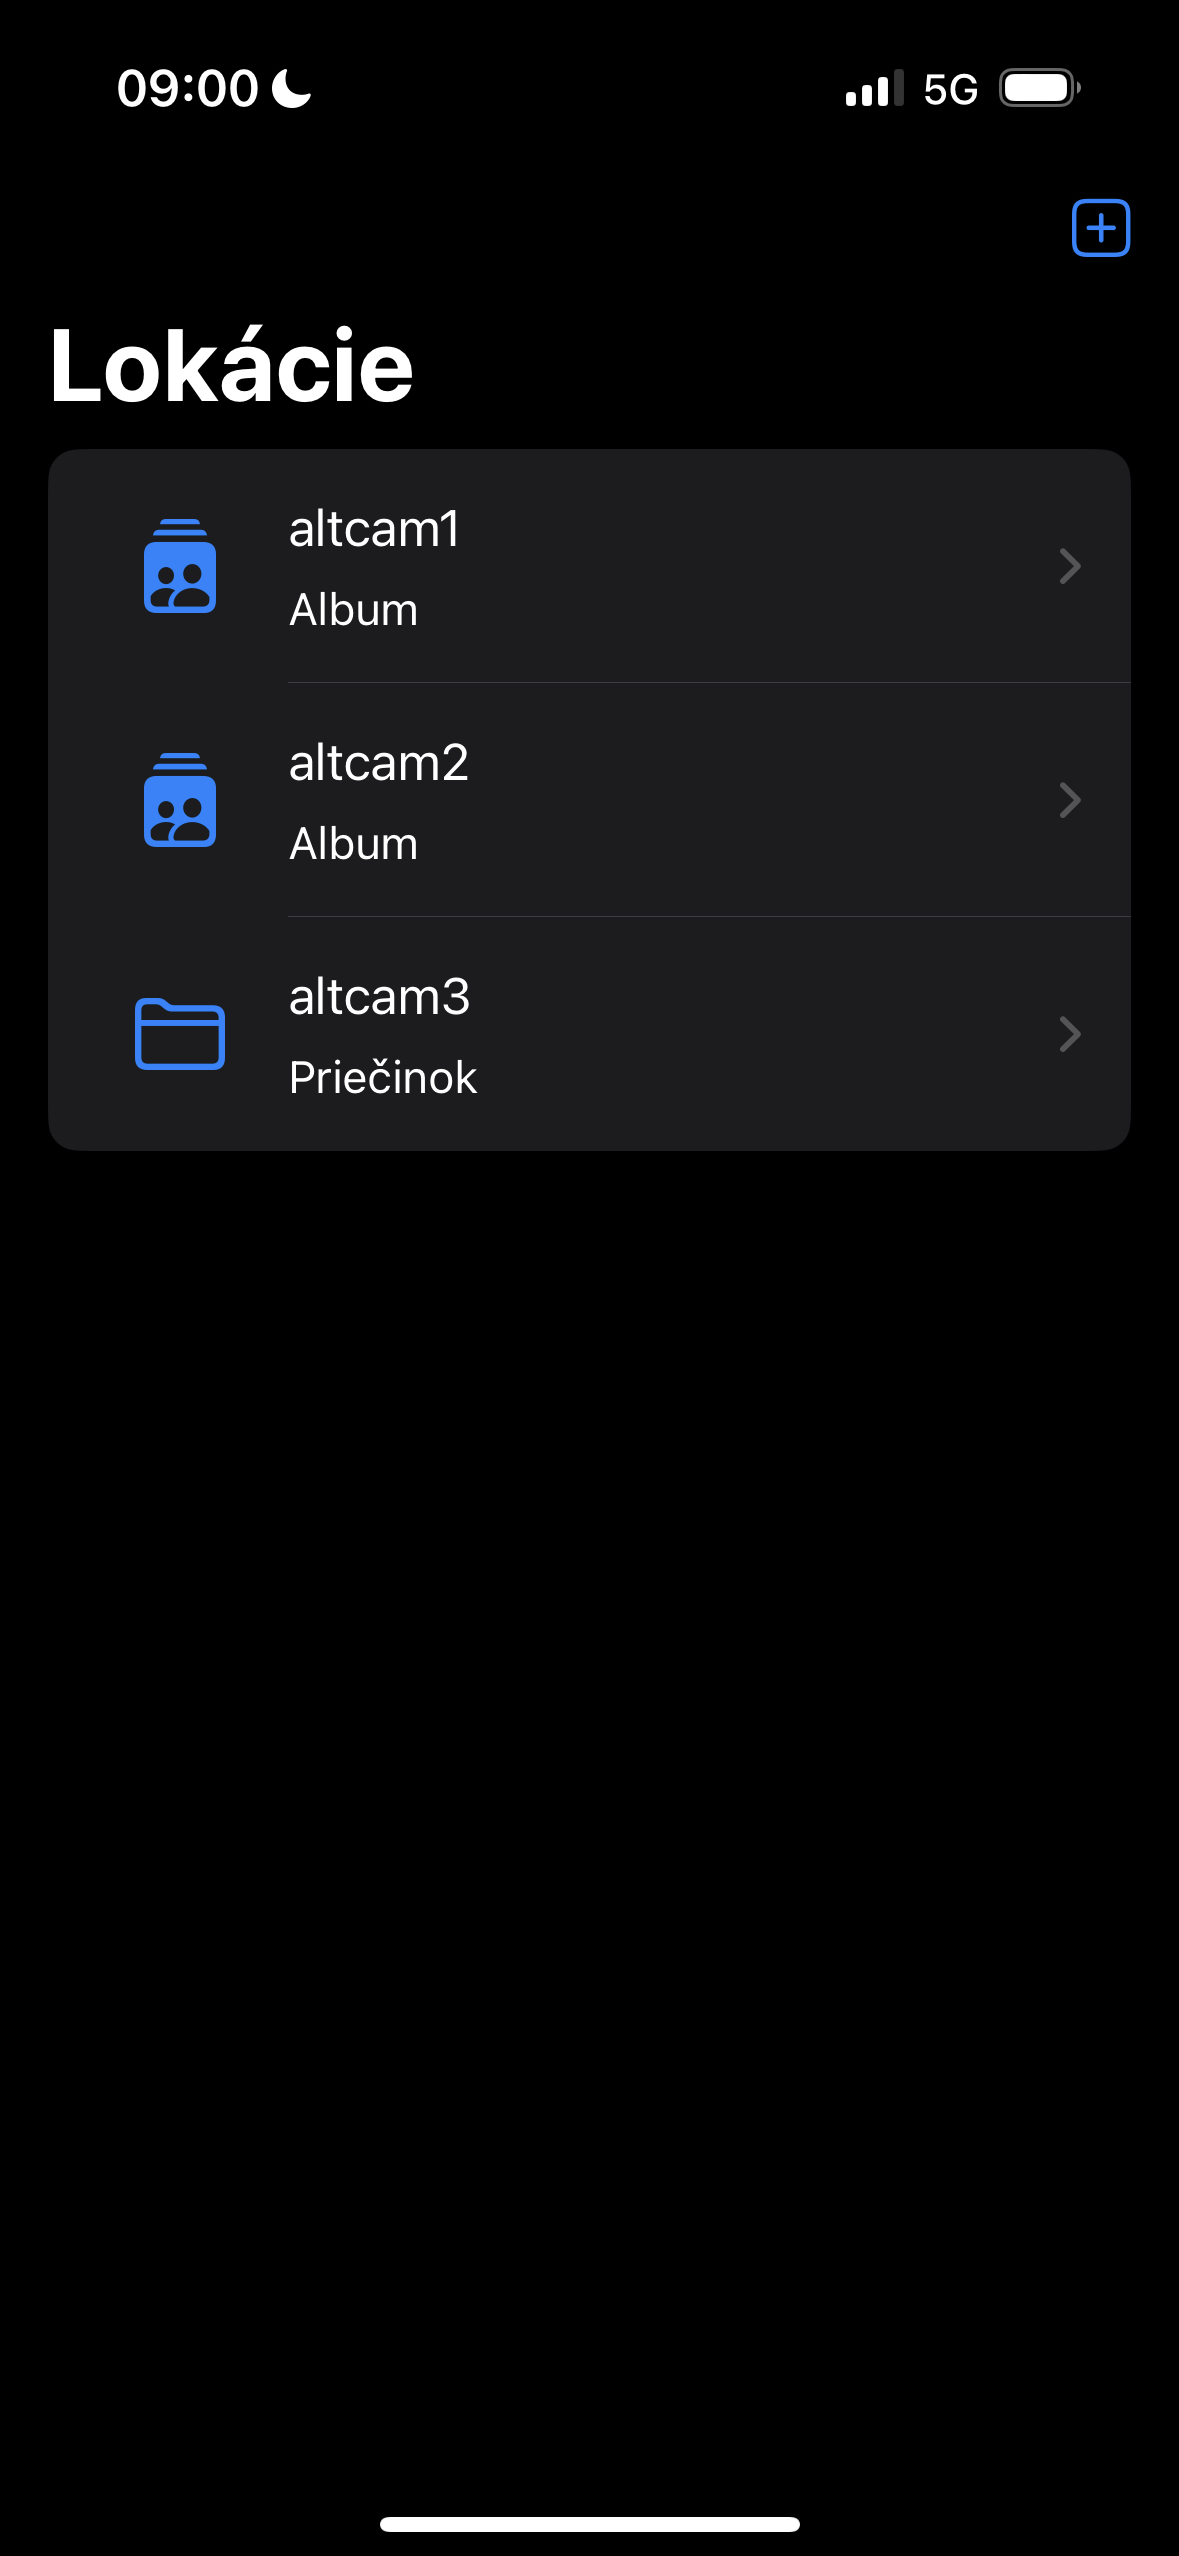
\includegraphics[width=4.5cm]{uvod.jpeg}
\end{center}

\pagebreak
\subsection{Vytváranie novej lokácie}
\begin{itemize}
\item[Navigačná lišta]{
	Navigačná lišta obsahuje názov obrazovky.
}
\item[Formulár]{
	Formulár vypĺňa celú obrazovku a obsahuje polia na voľbu typu lokácie, názov lokácie a potvrdzujúce tlačidlo.
}
\item[Typ lokácie]{
	Formulárová položka, ktorá po kliknutí otvorí natívne menu s výberom možností. Obsahuje možnosti {\tt Priečinok} a {\tt Album}. Predvolená možnosť je {\tt Priečinok}.
}
\item[Názov lokácie]{
	Formulárová položka, ktorá umožňuje zadať názov lokácie ako text v textovom poli.
}
\item[Potvrdzujúce tlačidlo]{
	Tlačidlo, ktoré potvrdí pridanie novej lokácie a uloží ju do pamäte cache zariadenia. Tlačidlo je vypnuté, ak nie je vyplnený názov lokácie.
}
\end{itemize}
\begin{center}
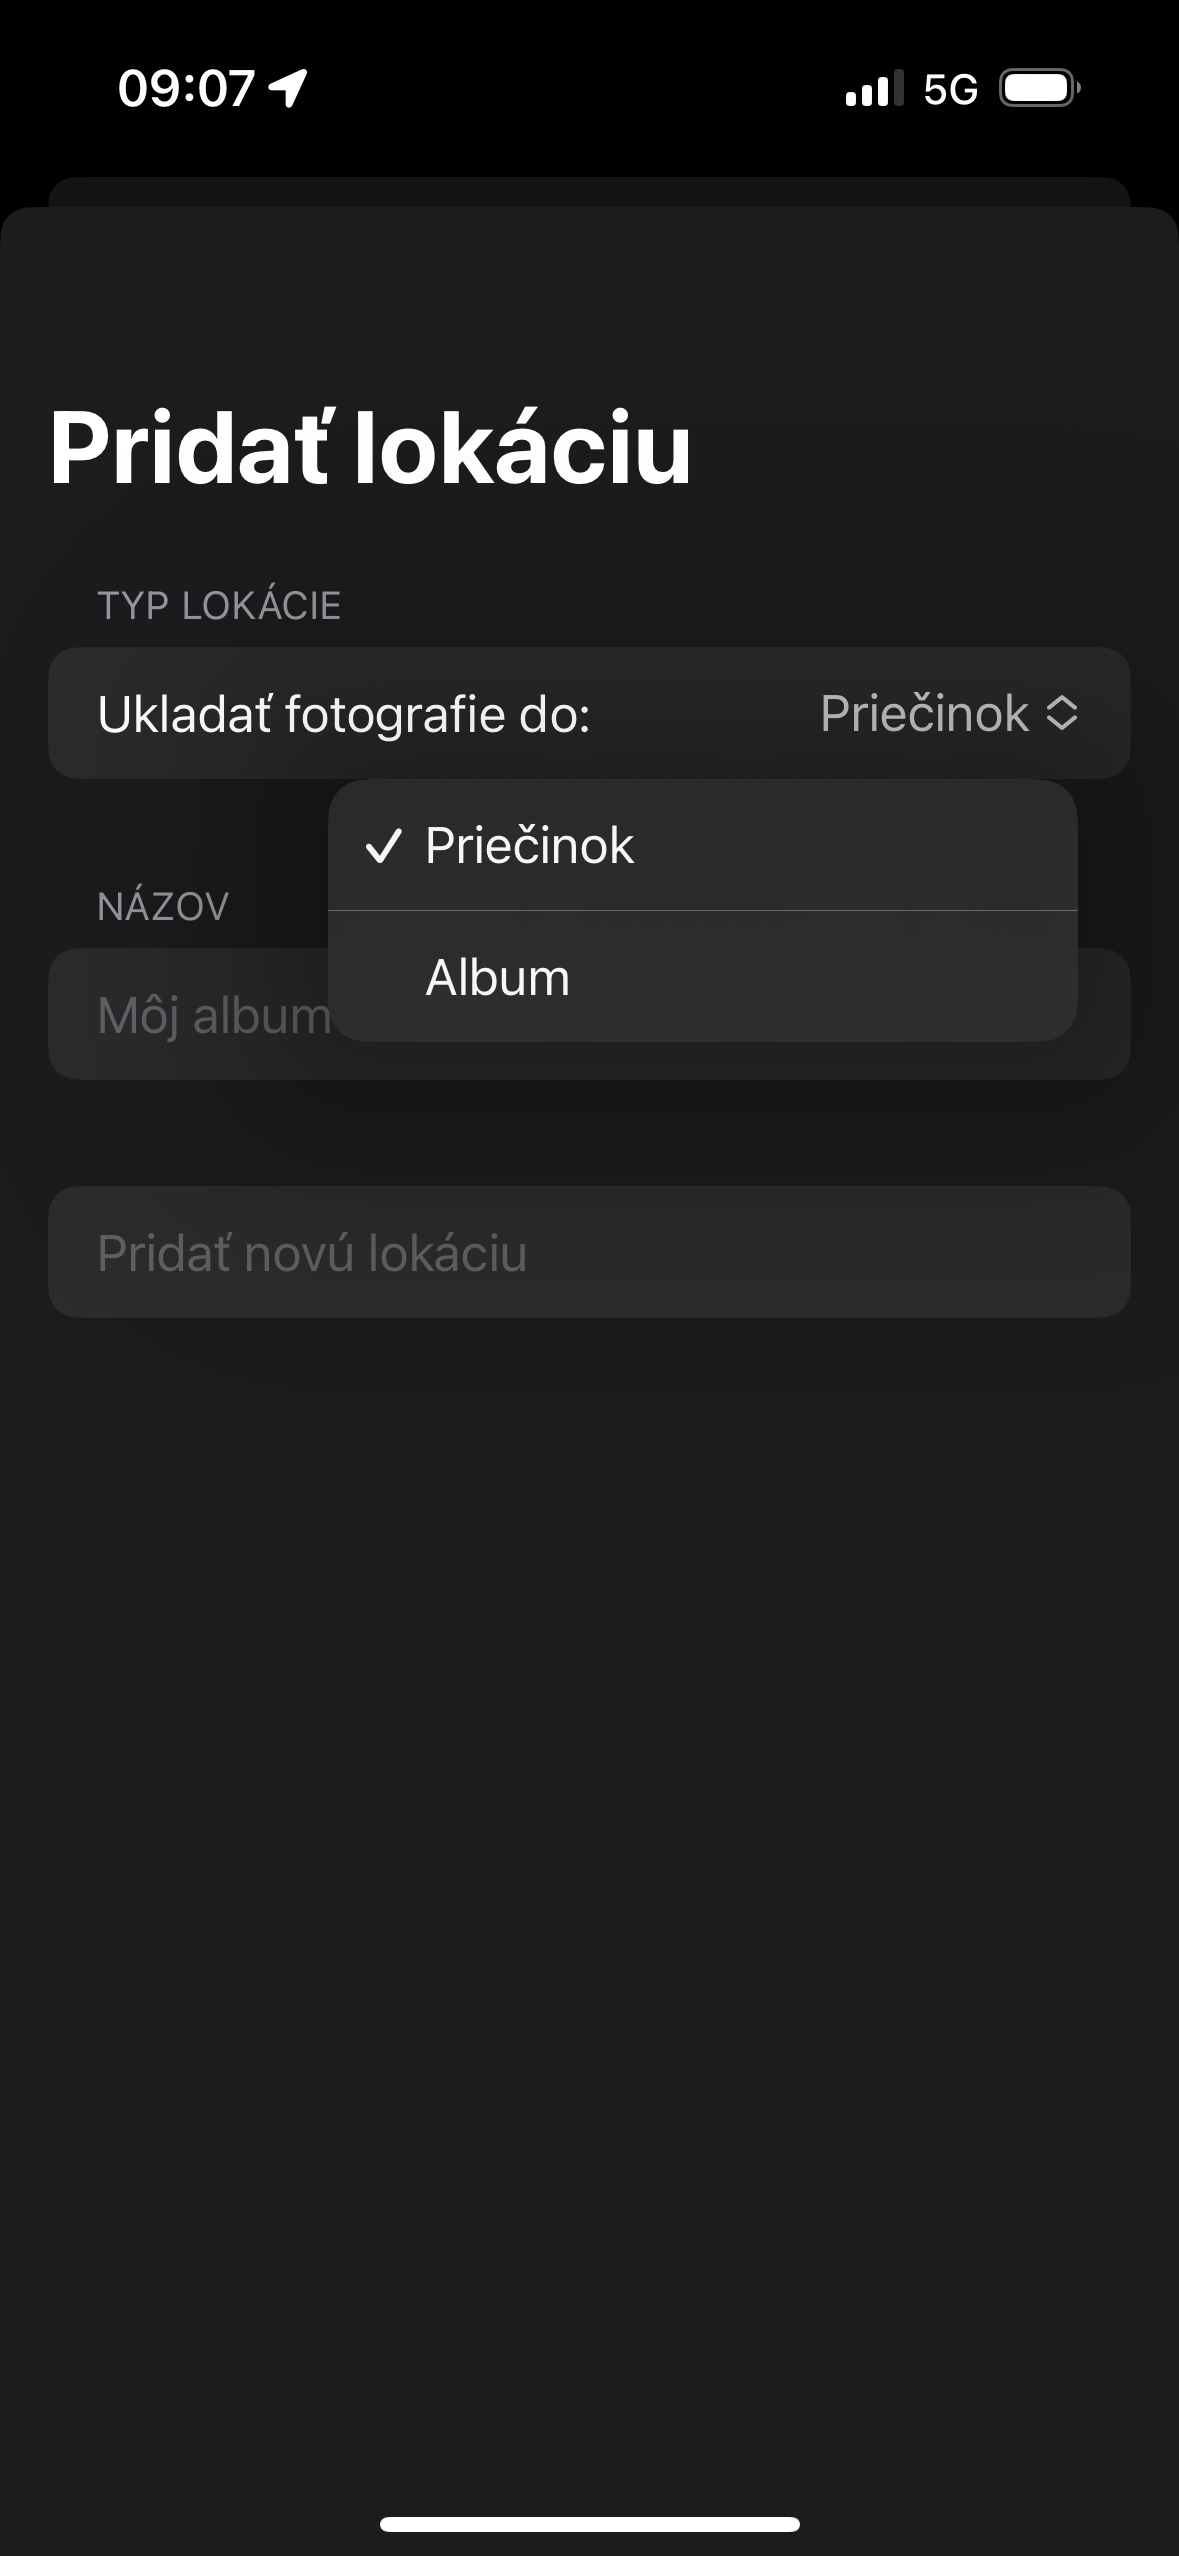
\includegraphics[width=4.5cm]{pridat.jpeg}
\end{center}

\pagebreak
\subsection{Kamera}
\begin{itemize}
\item[Navigačná lišta]{
	Navigačná lišta je priehľadná a obsahuje iba natívne tlačidlo späť. Tlačidlo späť vráti používateľa naspäť na výber lokácií.
}
\item[Náhľad kamery]{
	Náhľad kamery vypĺňa celú obrazovku od všetkých krajov. Zobrazuje vstup z kamery zariadenia. Obraz je roztiahnutý tak, aby vypĺňal celú plochu obrazovky zariadenia. Obraz je prispôsobený podľa aktuálneho nastavenia {\tt zoom}u.
}
\item[Zoom]{
	{\tt Náhľad kamery} podporuje rozpoznávanie gesta typu pinch (štipnutie). Gesto podľa pomeru vzdialeností začiatočných bodov a koncových bodov nastaví zmenu pomeru aktuálnej hodnoty {\tt zoom}u. Zoom sa nastaví ako parameter v kamere zariadenia (ak to je možné) a jeho zmena sa plynule animuje.
}
\item[Lišta akcií]{
	Lišta akcií obsahuje 3 hlavné akcie aplikácie. Na lište sa nachádzajú tlačidlá {\tt Galéria}, {\tt Odfotiť} a {\tt Otočiť}. Pozadie lišty akcií je priehľadné s efektom matného skla.
}
\item[Galéria]{
	Tlačidlo, ktoré po stlačení presmeruje používateľa do galérie. V prípade, že obrazovka bola otvorená s lokáciou typu {\tt Priečinok}, jedná sa o obrazovku {\tt Galéria}. V prípade, že obrazovka bola otvorená s lokáciou typu {\tt Album}, jedná sa o presmerovanie do systémovej galérie.
}
\item[Odfotiť]{
	Tlačidlo, ktoré po stlačení vyhotoví fotografiu. Podľa typu lokácie je fotografia uložená do požadovaného úložiska (priečinka alebo albumu). Fotografia je vyhotovená použitím základného nastavenia pre dané zariadenie. Po vyhotovení fotografie je používateľ upozornený vibračnou odozvou zariadenia.
}
\item[Otočiť]{
	Tlačidlo, ktoré po stlačení prepne aktívnu kameru zariadenia. Vyberie sa tá kamera, ktorá o sebe poskytuje informácie, že sa nachádza na opačnej strane zariadenia, než kamera, ktorá je aktuálne zvolená a vlastnosťami je najviac podobná kamere, ktorá bola zvolená doteraz.
}
\end{itemize}
\begin{center}
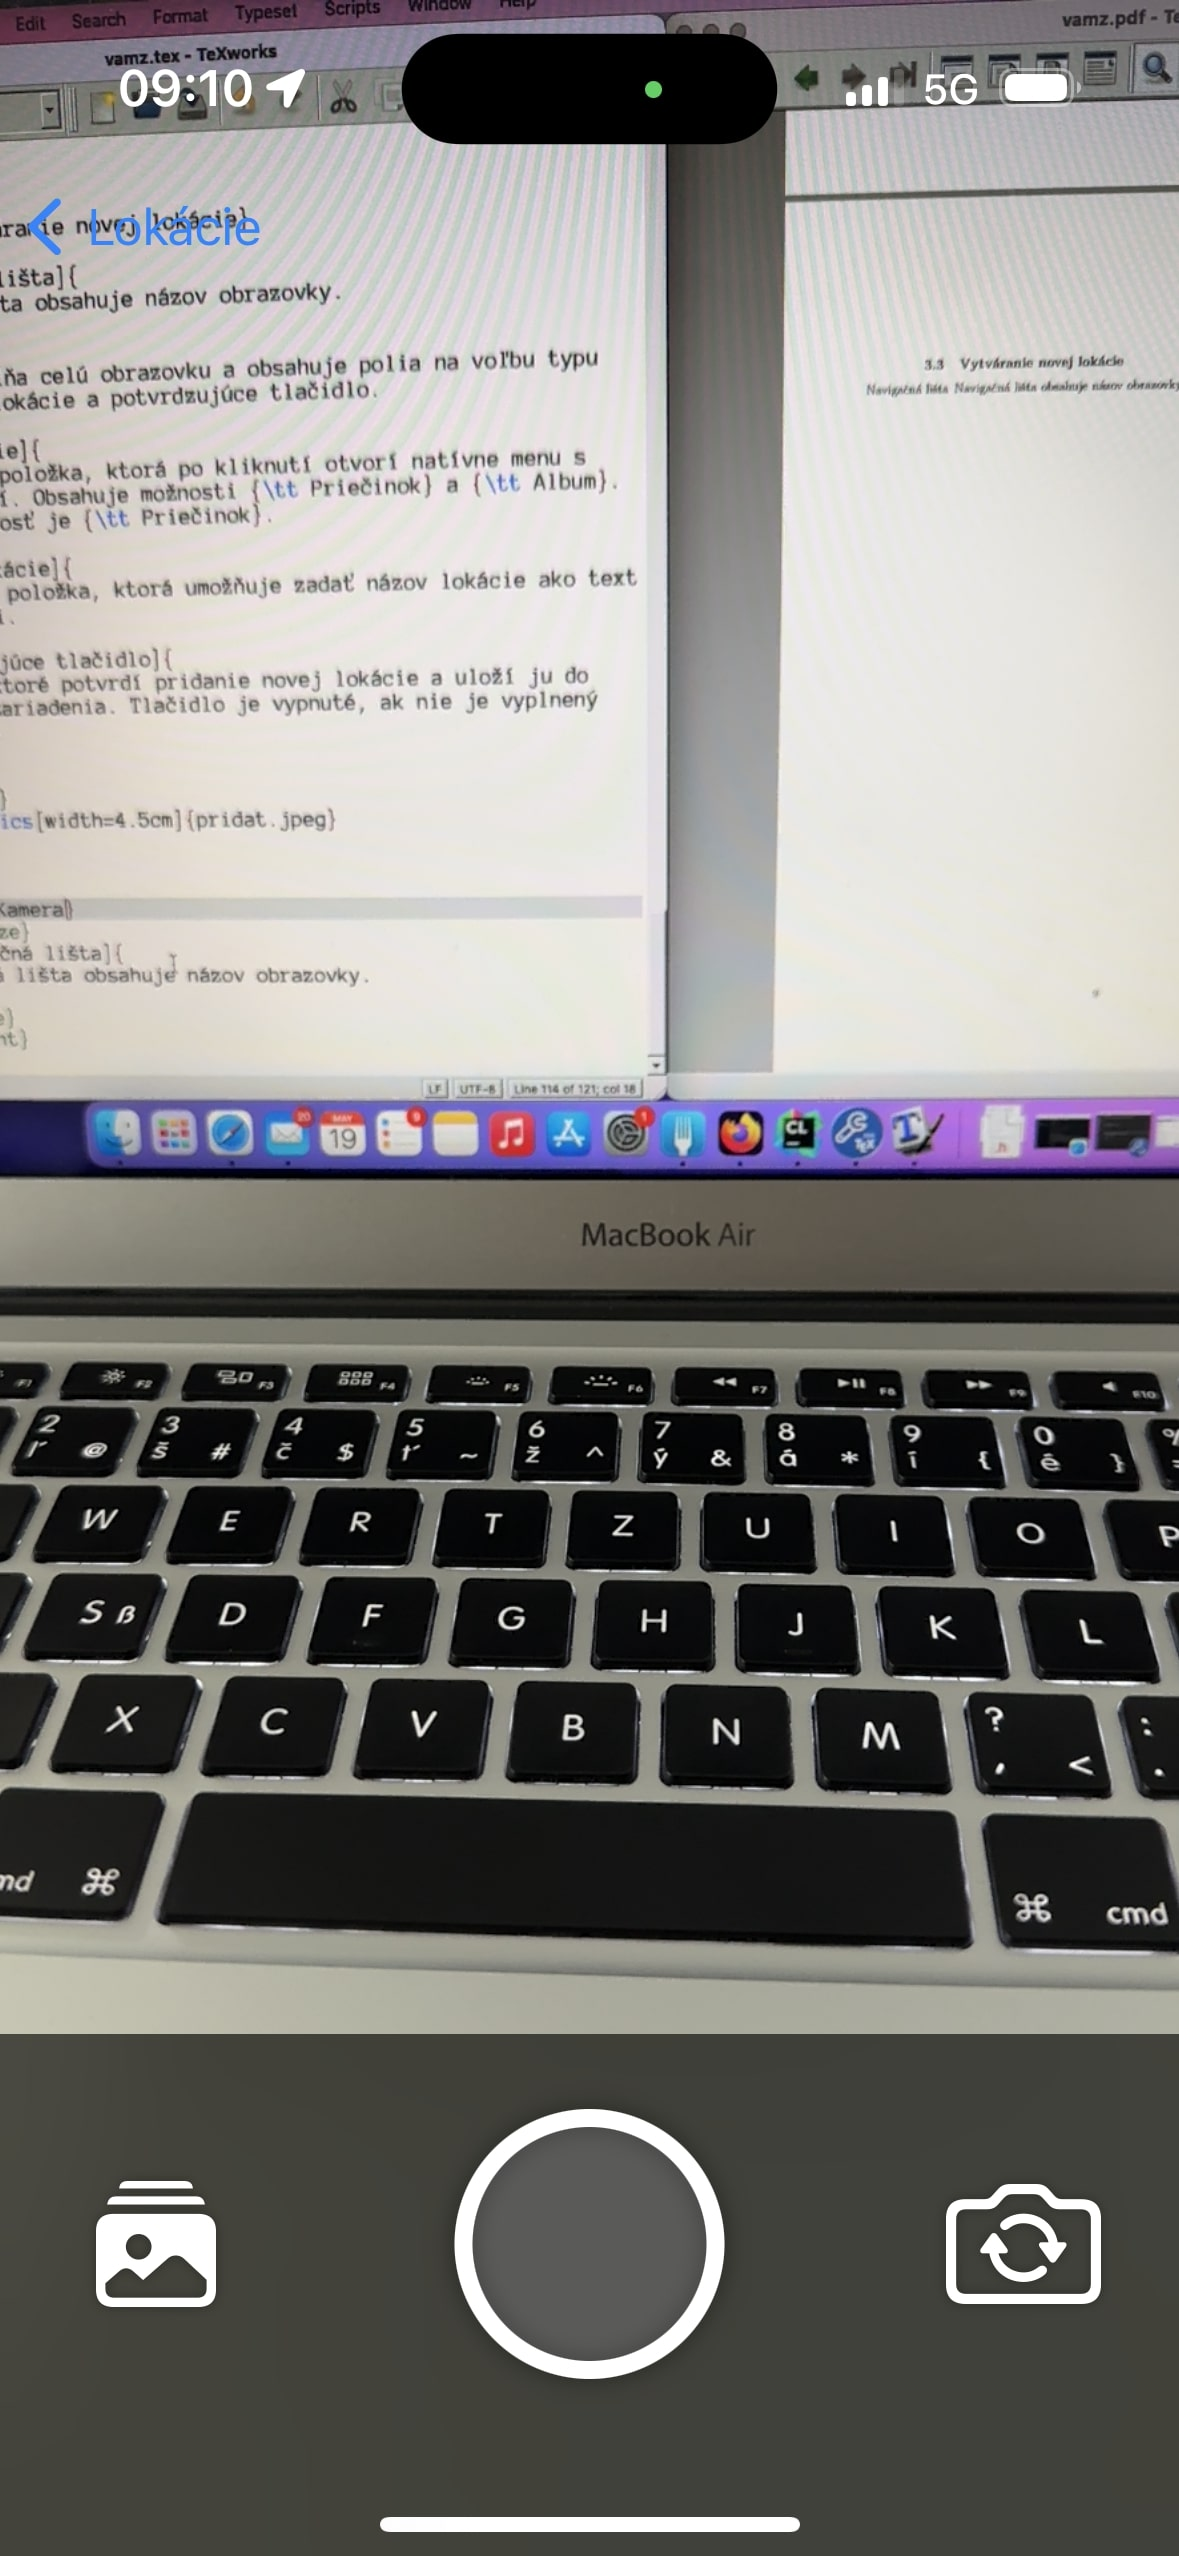
\includegraphics[width=4.5cm]{kamera.jpeg}
\end{center}

\pagebreak
\subsection{Galéria}
\begin{itemize}
\item[Navigačná lišta]{
	Navigačná lišta obsahuje natívne tlačidlo späť. V strede navigačnej lišty je správne vyskloňovaný text s počtom obrázkov v danom priečinku.
}
\item[Zoznam obrázkov]{
	Zoznam obrázkov vypĺňa celú obrazovku. Je rozdelený do 3 stĺpcov, obrázky sa do zoznamu dopĺňajú zhora nadol, zľava doprava. Obrázky reprezentujú fotografie, ktoré používateľ v danom priečinku vyhotovil. Po kliknutí na obrázok je používateľ presmerovaný na obrazovku {\tt Galéria - detail}, kde je daný obrázok predvolený.
}
\end{itemize}
\begin{center}
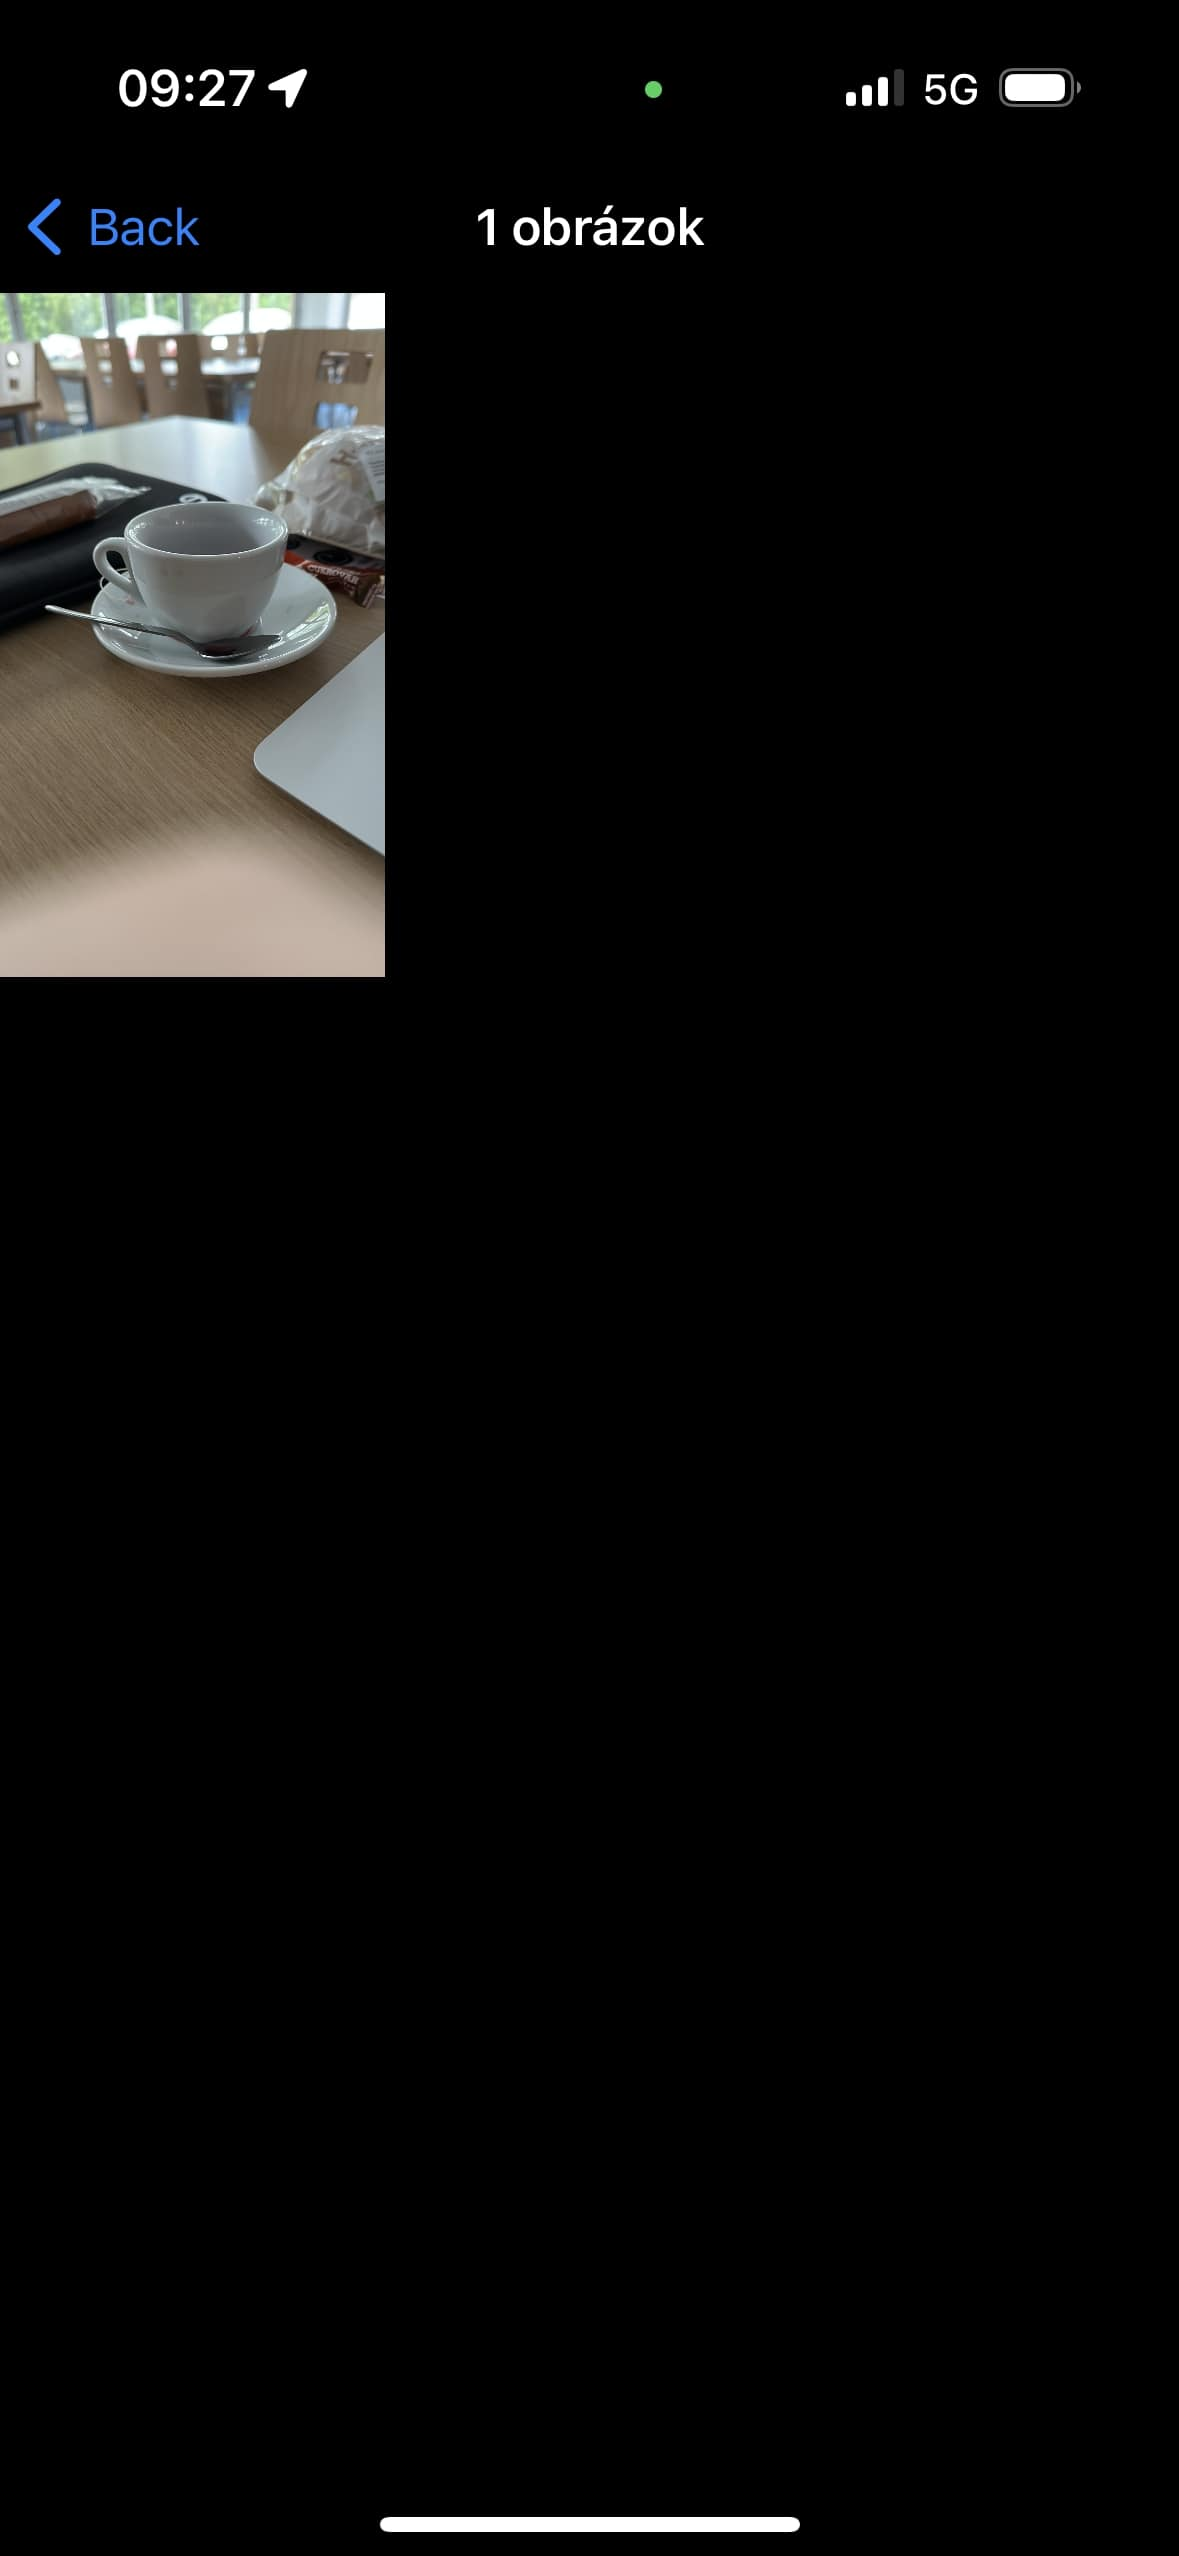
\includegraphics[width=4.5cm]{galeria.jpeg}
\end{center}

\pagebreak
\subsection{Galéria - detail}
\begin{itemize}
\item[Navigačná lišta]{
	Navigačná lišta obsahuje tlačidlo zatvoriť. Navigačná lišta je priehľadná. Po kliknutí kamkoľvek inam na obrazovku sa navigačná lišta skryje odanimovaním dohora.
}
\item[Obrázok]{
	Obrázok vypĺňa celú obrazovku. Dá sa gestami zväčšovať, zmenšovať a posúvať kamkoľvek po obrazovke. Celý obrázok sa dá odsunúť mimo obrazovky, v takom prípade sa na jeho miesto prisunie ďalší obrázok z galérie. Obrázky sa dajú posúvať a cyklovať dookola v nekonečnom cykle.
}
\item[Indikátor obrázka]{
	V spodnej časti obrazovky sa nachádza indikátor zvoleného obrázka. Ukazuje, ktorý obrázok v poradí je aktuálne zvolený, pomocou podfarbenej guličky.
}
\end{itemize}
\begin{center}

\includegraphics[width=4.5cm]{detail.jpeg}
\end{center}

\pagebreak
\section{Zoznam použitých zdrojov}
\begin{itemize}
\item {
	Apple developer dokumentácia - https://developer.apple.com/documentation/
}
\item {
	GoodPersistence knižnica - https://github.com/GoodRequest/GoodPersistence
}
\item {
	SharedObject knižnica - https://github.com/lorenzofiamingo/swiftui-shared-object
}
\end{itemize}
\end{document}
